% Drawing 141/01-10 -- folder 141, batch 01, archive page 11 (PDF page 12).
% Transcription: à droite de « $2 = 2\cdot 1$ », un bouquet de trois cercles : trois boucles issues d'un même gros point, vers le haut à droite, vers la droite et vers le bas.
% Kind: bouquet of three circles. Method 2 (schematic redraw from the facsimile). Status: ok.
% Notes: As on the page: three loops from one heavy point, each drawn as a closed curve leaving and returning to that point: one to the upper right, one to the right, one downwards. Nothing struck. Overlaid 2026-11-12 (Opus 5.5) on the 400 dpi colour crop: the three loops fall on the page within a unit; unchanged. Redrawn 2026-11-12 (issue 128): to check again.
% Coordinates: 1 unit = 0.4 mm = 1/100 of the crop width (bbox in page fractions: [0.32, 0.165, 0.42, 0.225]).
% Redrawn by Claude (claude-fable-5-2), issue #128, 2026-11-12; not checked by a human; not compiled (no TeX in the session).
% Overlaid by Claude (claude-opus-5-5) 2026-11-12 (issue #128): rasterised from its own coordinates over the 400 dpi colour facsimile and found to match it. Not compiled. Status: ok.
% Rights: reproduces part of the work -- behind RENDER_TRANSCRIPTS, never published by itself.
\documentclass[tikz,border=3pt]{standalone}
\usepackage{amsmath,amssymb}
\usetikzlibrary{patterns,arrows.meta}
\tikzset{pencil/.style={black!45}, struck/.style={black!35}, mpt/.style={circle,draw,inner sep=1.3pt}, pt/.style={circle,fill,inner sep=0.9pt}, opt/.style={circle,draw,fill=white,inner sep=1.1pt}}
\begin{document}
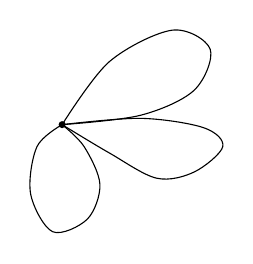
\begin{tikzpicture}[x=0.4mm,y=0.4mm,line cap=round,line join=round,font=\scriptsize]
\draw plot[smooth, tension=0.55] coordinates {(30,-43) (45,-23) (65,-13) (77,-19) (72,-32) (55,-40) (30,-43)};
\draw plot[smooth, tension=0.55] coordinates {(30,-43) (55,-41) (75,-44) (81,-50) (72,-58) (60,-60) (45,-52) (30,-43)};
\draw plot[smooth, tension=0.55] coordinates {(30,-43) (22,-50) (20,-65) (27,-77) (38,-73) (42,-62) (37,-50) (30,-43)};
\node[pt] at (30,-43) {};
\end{tikzpicture}
\end{document}
